\documentclass[aspectratio=169,12pt,professionalfonts]{beamer}
\usepackage{fontspec}
\usepackage{polyglossia}
\setdefaultlanguage{russian}
\setotherlanguage{english}
\setsansfont{Arial}
\setmainfont{Arial}
\newfontfamily\cyrillicfont{Arial}[Script=Cyrillic]
\newfontfamily\cyrillicfontsf{Arial}[Script=Cyrillic]
\newfontfamily\cyrillicfonttt{Arial}[Script=Cyrillic]
\usepackage{amsmath,amssymb,booktabs,tikz}
\usepackage{lmodern}
\geometry{paperwidth=192mm,paperheight=108mm}
\usetikzlibrary{arrows.meta,calc,positioning,patterns,decorations.pathmorphing}
\definecolor{ink}{HTML}{142D43}
\definecolor{teal}{HTML}{007F86}
\definecolor{gold}{HTML}{CE8429}
\definecolor{muted}{HTML}{617589}
\definecolor{paper}{HTML}{F7F8F6}
\definecolor{pale}{HTML}{E6EFEE}
\setbeamercolor{normal text}{fg=ink,bg=paper}
\setbeamercolor{frametitle}{fg=ink,bg=paper}
\setbeamercolor{structure}{fg=teal}
\setbeamercolor{alerted text}{fg=teal}
\setbeamercolor{block title}{fg=teal,bg=pale}
\setbeamercolor{block body}{fg=ink,bg=pale}
\setbeamerfont{frametitle}{size=\large,series=\bfseries}
\setbeamerfont{normal text}{size=\normalsize}
\setbeamersize{text margin left=8mm,text margin right=8mm}
\setbeamertemplate{navigation symbols}{}
\setbeamertemplate{itemize item}{\color{teal}\scriptsize$\bullet$}
\setlength{\parskip}{3pt}
\hyphenpenalty=10000
\exhyphenpenalty=10000
\setbeamertemplate{frametitle}{\vspace{2mm}\insertframetitle\par\vspace{1.5mm}{\color{teal}\hrule height .7pt}\vspace{1mm}}
\setbeamertemplate{footline}{\hfill\color{muted}\fontsize{7}{8}\selectfont
  \ifnum\value{framenumber}>\MainSlideCount Резерв\else\insertframenumber\,/\,\MainSlideCount\fi
  \hspace{8mm}\vspace{2mm}}
\hypersetup{colorlinks=true,urlcolor=teal,linkcolor=teal,
 pdftitle={От импульсов к пространству: корреляционная фемтоскопия},
 pdfauthor={Балинов Темир},pdfsubject={Вводная лекция, 19.10.2026}}
\urlstyle{same}

\newcommand{\takeaway}[1]{\par\vspace{4mm}{\large\color{teal}\textbf{#1}\par}}
\newcommand{\tagline}[1]{{\color{teal}\scriptsize\bfseries #1}\par}
\newcommand{\slidenote}[1]{\note{\input{notes/n#1.tex}}}
\newcommand{\hc}{\hbar c}
\newcommand{\dd}{\mathrm d}
\newcommand{\Lref}{Lisa et al. (2005)}
\newcommand{\Dref}{Anderson et al., NIM A 499, 659–678 (2003)}
\newcommand{\Kref}{А. Краева (STAR), Universe 10, 188 (2024)}
\newcommand{\chip}[2]{\colorbox{pale}{\parbox[c][12mm][c]{\dimexpr#1-2\fboxsep\relax}{\centering\small\color{ink}#2}}}
\newcommand{\prompt}[1]{{\color{teal}\large\bfseries #1}\par}
\newcommand{\measuretag}{\tagline{STAR · ЭКСПЕРИМЕНТ · Au+Au, 3 ГэВ}}
\tikzset{every node/.style={font=\small},arr/.style={-{Stealth[length=2mm]},thick},
  card/.style={rounded corners=2mm,draw=teal!30,fill=pale,align=center,inner sep=3mm},
  source/.style={circle,fill=teal,inner sep=2pt,text=white}}
\graphicspath{{figures/}}
\input{build/talk_metadata.tex}
\begin{document}
\section{Физическая задача}
{\setbeamercolor{background canvas}{bg=ink}\setbeamercolor{normal text}{fg=white}
\begin{frame}[plain]
\begin{tikzpicture}[remember picture,overlay]
\fill[teal!28!ink] ($(current page.north east)+(-5,0)$) rectangle (current page.south east);
\begin{scope}[shift={($(current page.east)+(-2.6,0)$)},scale=.65]
\draw[teal!75,line width=1pt] (0,0) ellipse (1 and 1.65);
\foreach \a in {0,25,...,350}{\draw[teal!70,opacity=.65] (0,0)--(\a:3.3);}
\foreach \a in {15,65,145,205,285}{\draw[gold,arr,line width=1.4pt] (0,0)--(\a:3.0);}
\fill[gold] (0,0) circle (.18);
\node[text=white] at (1.8,2.4) {$p_1$};\node[text=white] at (2.6,1.5) {$p_2$};
\end{scope}
\end{tikzpicture}
\color{white}
{\color{gold}\small ФИЗИЧЕСКИЙ ФАКУЛЬТЕТ МГУ\quad /\quad 19.10.2026}\par\vspace{7mm}
{\fontsize{23}{26}\selectfont\bfseries От импульсов\par к пространству}\par\vspace{3mm}
\begin{minipage}{.72\textwidth}
{\large Корреляционная фемтоскопия\par в столкновениях тяжёлых ядер}\par\vspace{4mm}
{\small Квантовая интерференция, статистический анализ\par и моделирование в SMASH}
\end{minipage}
\vfill{\small Балинов Темир\quad\color{white!65} Для студентов 1–2 курсов}
\slidenote{01}
\end{frame}}
\begin{frame}{Столкновения тяжёлых ядер: горячая плотная материя}
\begin{columns}[c,onlytextwidth]
\column{.53\textwidth}
\prompt{Горячая плотная материя.}
\vspace{7mm}
Каковы её размеры?\par\vspace{2mm}
Как она расширяется?
\column{.43\textwidth}
\begin{tikzpicture}[scale=.82]
\fill[teal!12] (0,0) circle(1.05);
\fill[gold!15] (2.7,0) circle(1.05);
\draw[teal,thick] (0,0) circle(1.05);
\draw[gold,thick] (2.7,0) circle(1.05);
\foreach \x/\y in {-.5/.3,.2/.6,.5/-.2,-.2/-.5,.2/0}{
\fill[teal!70] (\x,\y) circle(.13);
\fill[gold!75] (2.7+\x,\y) circle(.13);}
\draw[arr,teal] (-.7,1.35)--(.6,1.35);
\draw[arr,gold] (3.4,1.35)--(2.1,1.35);
\node[font=\scriptsize] at (1.35,1.85) {Два ядра Au};
\draw[arr,ink] (1.35,-1.2)--(1.35,-1.8);
\fill[pale] (1.35,-3) ellipse (1.65 and .9);
\draw[teal,thick] (1.35,-3) ellipse (1.65 and .9);
\foreach \x/\y in {0/0,-.7/.2,.6/.3,.9/-.2,-.4/-.4,.2/-.4}{
\fill[teal] (1.35+\x,-3+\y) circle(.07);}
\foreach \a in {0,45,135,180,225,315}{
\draw[arr,gold] ($(1.35,-3)+(\a:.7)$)--($(1.35,-3)+(\a:1.3)$);}
\node[font=\scriptsize,align=center] at (1.35,-4.6) {Взаимодействующая и\\расширяющаяся система};
\end{tikzpicture}
\end{columns}

\slidenote{02}
\end{frame}

\begin{frame}{Этапы столкновения и вымораживание частиц}
\begin{tikzpicture}[x=1cm,y=1cm]
\draw[arr,ink] (.2,0)--(16.2,0) node[below left,font=\scriptsize] {время};
\foreach \x/\a/\b in {1/{Перекрытие}/{ядер},5/{Плотная}/{среда},9.2/{Химическое}/{вымораживание},13.8/{Кинетическое}/{вымораживание}}{
\fill[teal] (\x,0) circle (.07);\node[align=center,font=\small\bfseries] at (\x,-.65) {\a\\\b};}
\draw[teal,thick,fill=teal!10] (.8,1.8) ellipse (.15 and .65);
\draw[gold,thick,fill=gold!15] (1.2,1.8) ellipse (.15 and .65);
\fill[gold!50] (5,1.8) ellipse (.85 and .7);
\draw[teal,fill=teal!10,thick] (9.2,1.8) ellipse (1.1 and .75);
\foreach \a in {0,45,...,315}{\fill[teal] ($(9.2,1.8)+(\a:.65)$) circle (.055);}
\foreach \a in {0,35,...,350}{\fill[teal] ($(13.8,1.8)+(\a:1.05)$) circle (.045);
\draw[arr,gold] ($(13.8,1.8)+(\a:1.1)$)--($(13.8,1.8)+(\a:1.55)$);}
\end{tikzpicture}
\vspace{3mm}
\begin{columns}[T,onlytextwidth]
\column{.47\textwidth}\tagline{ХИМИЧЕСКОЕ}\textbf{Состав частиц} почти не меняется.
\column{.49\textwidth}\tagline{КИНЕТИЧЕСКОЕ}Частицы \textbf{перестают рассеиваться}.
\end{columns}
\takeaway{Фемтоскопия характеризует область испускания пионов.}

\slidenote{03}
\end{frame}
\begin{frame}{Импульсы измерены, точки испускания неизвестны}
\begin{columns}[c,onlytextwidth]
\column{.48\textwidth}
\begin{tikzpicture}[scale=.95]
\fill[pale] (0,0) ellipse (1.5 and 1.05);
\draw[teal,dashed,thick] (0,0) ellipse (1.5 and 1.05);
\node[text=teal,font=\Huge] at (0,0) {?};
\draw[arr,teal,line width=1.4pt] (1,.4)--(3.7,1.6) node[right] {$\mathbf p_1$};
\draw[arr,gold,line width=1.4pt] (1,-.4)--(3.7,-1.3) node[right] {$\mathbf p_2$};
\node[font=\small,align=center] at (0,-1.8) {Область\\испускания};
\node[font=\scriptsize,text=muted] at (0,1.65) {Размер? Время?};
\end{tikzpicture}
\column{.48\textwidth}
\prompt{Импульсы известны.}
По траекториям частиц.
\par\vspace{4mm}
\prompt{Координаты неизвестны.}
Разрешения детектора недостаточно\par для фемтометровых расстояний.
\[1\ \text{фм}=10^{-15}\ \text{м}.\]
\end{columns}
\takeaway{Корреляции импульсов содержат информацию о размерах.}

\slidenote{04}
\end{frame}
\section{От звезды к пионным парам}
\begin{frame}{HBT: измерение углового размера звезды}
\tagline{1956 / ХЭНБЕРИ БРАУН И ТВИСС (HBT)}
\begin{tikzpicture}[x=1cm,y=1cm]
\fill[gold!30] (1.4,1.6) circle(.65);\draw[gold!80!black,thick] (1.4,1.6) circle(.65);
\node[font=\small] at (1.4,.55) {Звезда};
\node[card,text width=2.5cm] (a) at (8.0,3.0) {Приёмник 1\\$I_1(t)$};
\node[card,text width=2.5cm] (b) at (8.0,.2) {Приёмник 2\\$I_2(t)$};
\draw[arr,teal] (2,1.9)--(a.west);\draw[arr,teal] (2,1.3)--(b.west);
\draw[<->,muted] (6.1,.3)--node[left] {$d$}(6.1,2.9);
\node[card,text width=3.2cm,minimum height=20mm] (c) at (13.5,1.6) {Сравниваем\\флуктуации\\интенсивности};
\draw[arr,ink] (a.east)--(c.north west);\draw[arr,ink] (b.east)--(c.south west);
\end{tikzpicture}\par\vspace{2mm}
\begin{center}
Угловой размер определяют по зависимости корреляции\par
от расстояния $d$ между приёмниками.
\end{center}
\slidenote{05}
\end{frame}
\begin{frame}{Корреляции фотонов и тождественных пионов}
\begin{columns}[T,onlytextwidth]
\column{.29\textwidth}
\tagline{1956 / ОПТИКА}
\begin{tikzpicture}[scale=.8]
\fill[gold!35] (0,0) circle(.42);
\node[card] (a) at (3,1) {$I_1$};\node[card] (b) at (3,-1) {$I_2$};
\draw[arr,teal] (.4,.2)--(a);\draw[arr,teal] (.4,-.2)--(b);
\end{tikzpicture}\par
Фотоны: корреляция\par интенсивностей.
\column{.32\textwidth}
\tagline{1960 / ПИОННЫЕ КОРРЕЛЯЦИИ}
\[\overline p+p\longrightarrow\pi\pi\ldots\]
\[{\color{teal}\pi^+\pi^+}\quad\text{или}\quad{\color{teal}\pi^-\pi^-}.\]
Пионы: корреляции\par тождественных бозонов.
\column{.31\textwidth}
\tagline{1970-е / КОПЫЛОВ–ПОДГОРЕЦКИЙ}
\begin{tikzpicture}[scale=.8]
\fill[pale] (0,0) ellipse (1.1 and .7);
\foreach \a in {0,45,...,315}{\draw[arr,teal] (\a:.5)--(\a:1.35);}
\end{tikzpicture}\par
Корреляция $\leftrightarrow$\par пространство и время\par испускания.
\end{columns}

\slidenote{06}
\end{frame}
\section{Почему корреляция связана с размером}
\begin{frame}{Двухчастичные корреляции дополняют спектры}
\begin{columns}[c,onlytextwidth]
\column{.57\textwidth}\tagline{УЧЕБНЫЙ СПЕКТР}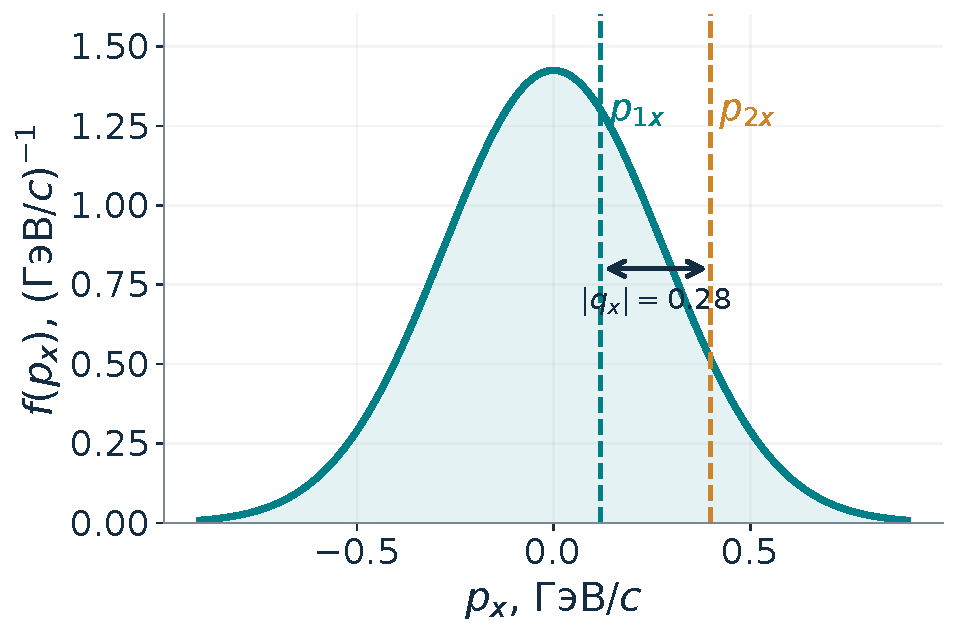
\includegraphics[width=\linewidth]{single_spectrum.pdf}
\column{.39\textwidth}
\tagline{ОДНА ЧАСТИЦА}
$f(\mathbf p)$: какие импульсы\par встречаются часто?\par\vspace{3mm}
\tagline{ДВЕ ЧАСТИЦЫ}
$f_2(\mathbf p_1,\mathbf p_2)$:\par какие встречаются \textbf{вместе}?\par\vspace{3mm}
\[C=\mathcal N\frac{f_2}{f(\mathbf p_1)f(\mathbf p_2)}.\]
При независимом испускании: $C=1$.
\end{columns}

\slidenote{07}
\end{frame}
\begin{frame}{Разность и полусумма импульсов пары}
\begin{columns}[c,onlytextwidth]
\column{.50\textwidth}
\[\boxed{\mathbf q=\mathbf p_1-\mathbf p_2}.\]
\[\mathbf K=\frac{\mathbf p_1+\mathbf p_2}{2},\qquad k_T=|\mathbf K_T|.\]
\vspace{2mm}
$\mathbf q$: разность импульсов.\par\vspace{2mm}
$\mathbf K$: средний импульс пары.
\column{.46\textwidth}
\begin{tikzpicture}[scale=1.15]
\draw[arr,teal,line width=1.7pt] (0,0)--(3,1.4) node[right] {$\mathbf p_{1T}$};
\draw[arr,gold!85!black,line width=1.7pt] (0,0)--(2.5,.3) node[right] {$\mathbf p_{2T}$};
\draw[arr,ink] (2.5,.3)--(3,1.4) node[midway,right=1.5mm] {$\mathbf q_T$};
\draw[arr,ink,dashed] (0,0)--(2.75,.85);
\node[font=\small] at (1.6,-.55) {Пунктир: $\mathbf K_T$};
\end{tikzpicture}
\end{columns}

\slidenote{08}
\end{frame}
\begin{frame}{Неразличимость пионов и квантовая интерференция}
\begin{columns}[c,onlytextwidth]
\column{.68\textwidth}
\begin{tikzpicture}[x=1cm,y=1cm]
\fill[pale] (-.45,-.6) rectangle (.45,2.6);
\node[source] (a) at (0,2) {$A$};\node[source] (b) at (0,0) {$B$};
\node[card] (p1) at (6.5,2) {$p_1$};\node[card] (p2) at (6.5,0) {$p_2$};
\draw[arr,teal,line width=1.5pt] (a)--(p1);\draw[arr,teal,line width=1.5pt] (b)--(p2);
\draw[arr,gold,dashed,line width=1.5pt] (a)--(p2);\draw[arr,gold,dashed,line width=1.5pt] (b)--(p1);
\node[teal,font=\small] at (3.2,2.6) {Первый вариант};
\node[gold,font=\small] at (3.2,-.7) {Перестановка пионов};
\node[font=\scriptsize,align=center] at (0,-1.4) {точки\\испускания};
\node[font=\scriptsize,align=center] at (6.5,-1.4) {конечные\\импульсы};
\end{tikzpicture}
\column{.28\textwidth}
{\Large $\pi^+\pi^+$}\par\vspace{3mm}
Какой пион\par пришёл из $A$?\par\vspace{3mm}
Варианты\par\textbf{неразличимы.}
\end{columns}

\slidenote{09}
\end{frame}
\begin{frame}{Амплитуда пары тождественных пионов}
\begin{columns}[c,onlytextwidth]
\column{.28\textwidth}
\tagline{ПЕРВЫЙ ВАРИАНТ}
$A\to p_1$,\quad $B\to p_2$
\column{.68\textwidth}
\[a=\exp\!\left[-\frac{i}{\hc}\left(p_1\cdot x_A+p_2\cdot x_B\right)\right]\]
\end{columns}
\vspace{3mm}
\begin{columns}[c,onlytextwidth]
\column{.28\textwidth}
{\color{gold!85!black}\scriptsize\bfseries ПЕРЕСТАНОВКА ПИОНОВ}\par
$A\to p_2$,\quad $B\to p_1$
\column{.68\textwidth}
\[b=\exp\!\left[-\frac{i}{\hc}\left(p_2\cdot x_A+p_1\cdot x_B\right)\right]\]
\end{columns}
\vspace{3mm}
\[\boxed{\Psi=\frac{a+b}{\sqrt2}},\qquad |a|=|b|=1.\]
\begin{center}
\small $p^\mu=(E,\mathbf p)$; $x^\mu=(ct,\mathbf r)$; $p\cdot x=Ect-\mathbf p\cdot\mathbf r$; $c=1$.\par
$p$ — ГэВ, $x$ — фм; $\hc\simeq0.197$ ГэВ·фм.
\end{center}
\slidenote{10}
\end{frame}
\begin{frame}{От суммы амплитуд к интерференционному члену}
\[|\Psi|^2=\frac{|a|^2+|b|^2+ab^*+a^*b}{2}
           =1+\operatorname{Re}(ab^*).\]
\vspace{2mm}
\[
\begin{aligned}
ab^*&=\exp\!\left[-\frac{i}{\hc}\Bigl(p_1\cdot x_A+p_2\cdot x_B
                       -p_2\cdot x_A-p_1\cdot x_B\Bigr)\right]\\[2mm]
    &=\exp\!\left[-\frac{i}{\hc}(p_1-p_2)\cdot(x_A-x_B)\right]=e^{-i\varphi}.
\end{aligned}
\]
\vspace{2mm}
\[q^\mu=p_1^\mu-p_2^\mu,\qquad\Delta x=x_A-x_B,\qquad\varphi=\frac{q\cdot\Delta x}{\hc}.\]
\[\boxed{|\Psi|^2=1+\cos\varphi}\]
\begin{center}\small $*$ — комплексное сопряжение; $\operatorname{Re}$ — действительная часть.\par
При $q\to0$ относительная вероятность стремится к 2.\end{center}
\slidenote{11}
\end{frame}
\begin{frame}{Корреляция и распределение точек испускания}
\begin{columns}[c,onlytextwidth]
\column{.34\textwidth}
\begin{tikzpicture}[scale=.9]
\fill[pale] (0,0) ellipse (2 and 1.55);
\foreach \x/\y in {-1/.4,-.4/1,.1/-.4,.9/.7,1.4/-.6,-1.2/-.6,.4/.2}{\fill[teal] (\x,\y) circle(.09);}
\node[source] (a) at (-.4,1) {$A$};\node[source] (b) at (1.4,-.6) {$B$};
\draw[<->,gold,thick] (a)--(b);
\node[align=center,font=\small] at (0,-2.6) {$\rho(x;K)$\\распределение испускания\\[2mm]$\int\dd^4x\,\rho(x;K)=1$};
\end{tikzpicture}
\column{.62\textwidth}
{\large Усредняем по точкам источника}
\[C(q,K)\simeq\bigl\langle|\Psi|^2\bigr\rangle=1+\langle\cos\varphi\rangle.\]
\[\boxed{C-1\simeq\left|\int\dd^4x\,\rho(x;K)e^{iq\cdot x/\hc}\right|^2}\]
\vspace{3mm}
\small Независимое испускание.\par Взаимодействием между пионами\par после испускания пренебрегаем.
\end{columns}
\slidenote{12}
\end{frame}
\begin{frame}{Чем больше источник, тем уже корреляционный пик}
\begin{columns}[c,onlytextwidth]
\column{.60\textwidth}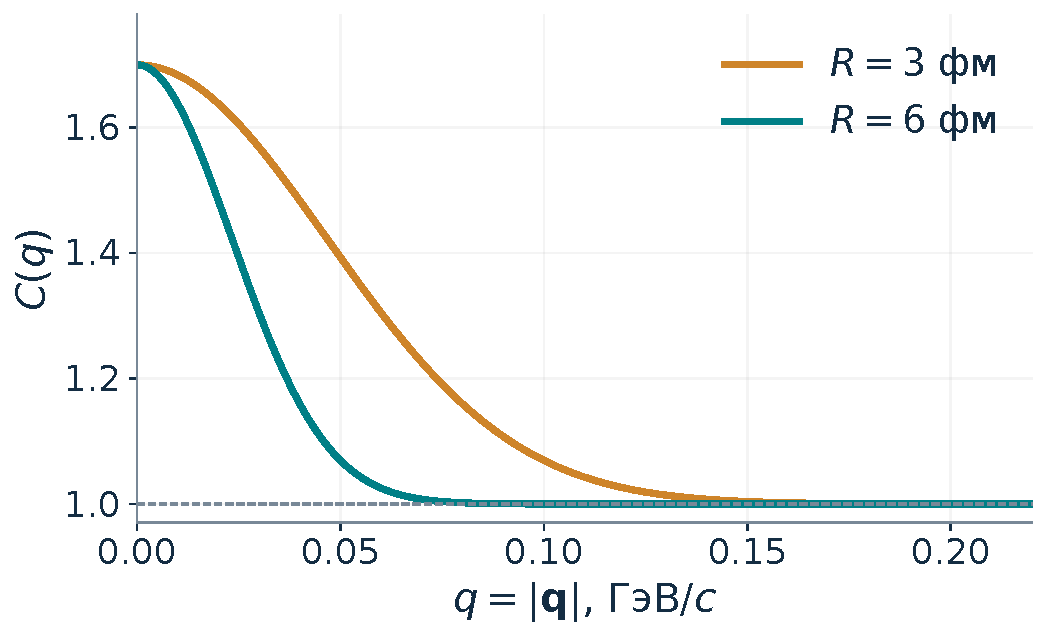
\includegraphics[width=\linewidth]{gaussian_radii.pdf}
\column{.36\textwidth}
\tagline{УЧЕБНЫЙ ГАУССОВ ИСТОЧНИК}
\[C=1+\lambda e^{-R^2q^2/(\hc)^2}.\]
\[{\color{teal}\Delta q\sim\frac{\hc}{R}}.\]
\small $R$: среднеквадратичный\par размер по одной оси.\par\vspace{2mm}
$\lambda$: высота пика\par над уровнем $C=1$.
\end{columns}


\slidenote{13}
\end{frame}
\section{Как это измеряют в STAR}
\begin{frame}{Время-проекционная камера (TPC)}
\begin{columns}[c,onlytextwidth]
\column{.56\textwidth}
\begin{tikzpicture}[x=1cm,y=1cm]
\fill[teal!5] (0,.5) rectangle (6.6,4.1);
\draw[teal!45,thick] (0,.5) rectangle (6.6,4.1);
\fill[gold!30] (0,.15) rectangle (6.6,.5);
\foreach \x in {.2,.7,...,6.4}{\draw[muted!55] (\x,.15)--(\x,.5);}
\draw[gold!80!black,line width=1.5pt] (.7,3.7)--(5.9,2.6);
\foreach \x/\y in {1/3.64,1.9/3.45,2.8/3.26,3.7/3.07,4.6/2.88,5.5/2.69}{
\fill[teal] (\x,\y) circle(.055);
\draw[arr,teal,dashed] (\x,\y-.12)--(\x,.65);}
\node[font=\scriptsize,text=gold!70!black] at (2.8,4.5) {Заряженная частица ионизует газ};
\node[font=\scriptsize,fill=paper,inner sep=1mm] at (3.3,1.8) {Дрейф электронов};
\node[font=\scriptsize] at (3.3,-.22) {Торцевая плоскость считывания: площадки $(x,y)$};
\draw[arr,ink] (-.45,.6)--(-.45,3.9) node[above] {$z$};
\draw[arr,muted] (7,2.7)--(7,3.8) node[above] {$\mathbf E,\mathbf B$};

\end{tikzpicture}
\column{.40\textwidth}
{\bfseries По ионизации восстанавливаем\par траекторию частицы.\par}\par\vspace{3mm}
Площадки $\to (x,y)$.\par Время дрейфа $\to z$.
\par\vspace{2mm}
Трек — восстановленная\par траектория частицы.
\end{columns}


\slidenote{14}
\end{frame}
\begin{frame}{Импульс и ионизационные потери частицы в TPC}
\begin{columns}[c,onlytextwidth]
\column{.45\textwidth}
\begin{tikzpicture}[scale=1.05]
\draw[muted!25] (0,0) grid[step=.5] (3.1,2.9);
\draw[arr,gold!85!black,very thick] (0,0) arc[start angle=-90,end angle=10,radius=1.4];
\draw[arr,teal,very thick] (0,0) arc[start angle=-90,end angle=-32,radius=3];
\fill[ink] (0,0) circle(.05);
\node[text=teal,font=\scriptsize] at (2.6,1.0) {больший $p_T$};
\node[text=gold!75!black,font=\scriptsize] at (1.1,2.2) {меньший $p_T$};
\node[font=\small] at (2.7,2.65) {$\mathbf B\;\otimes$};
\node[font=\scriptsize,text=muted] at (1.6,-.5) {Поперечная плоскость};
\end{tikzpicture}
\[p_T[\text{ГэВ}/c]\simeq0.30\,|Q/e|\,B[\text{Т}]\,r[\text{м}].\]

\column{.51\textwidth}
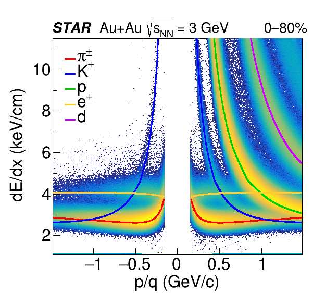
\includegraphics[width=\linewidth,height=56mm,keepaspectratio]{kraeva_2024_pid_tpc_dedx.pdf}\par
\small При известном $p$ сравниваем $dE/dx$\par с расчётными значениями для $\pi$, $K$, $p$.
\end{columns}

\slidenote{15}
\end{frame}
\begin{frame}{Времяпролётная система (TOF)}
\begin{columns}[c,onlytextwidth]
\column{.44\textwidth}
\begin{tikzpicture}[x=1cm,y=1cm]
\node[source] (a) at (.2,0) {$t_0$};
\node[card] (b) at (5.3,0) {$t_{\rm hit}$};
\draw[arr,teal,thick] (a) to[bend left=22] node[above] {длина пути $L$} (b);
\node[font=\scriptsize] at (.2,-.7) {событие};\node[font=\scriptsize] at (5.3,-.7) {TOF};
\end{tikzpicture}
\[\Delta t=t_{\rm hit}-t_0,\qquad\beta=\frac{L}{c\Delta t}.\]
\[\boxed{m^2=p^2(\beta^{-2}-1)}\quad(c=1).\]

\column{.52\textwidth}
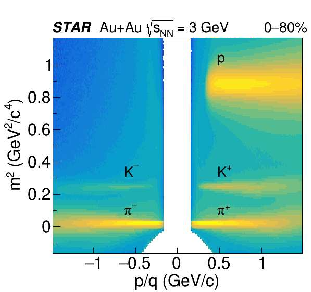
\includegraphics[width=\linewidth,height=56mm,keepaspectratio]{kraeva_2024_pid_tof_mass2.pdf}\par
\small Импульс + скорость $\to$ оценка массы\par $\to$ отбор пионов.
\end{columns}


\slidenote{16}
\end{frame}
\begin{frame}{STAR: столкновения ядер золота при 3 ГэВ}
\begin{columns}[c,onlytextwidth]
\column{.60\textwidth}
\begin{tikzpicture}[x=1cm,y=1cm]
\fill[pale,rounded corners] (.3,-1.5) rectangle (9,1.7);
\draw[teal!40,thick] (.3,-1.5) rectangle (9,1.7);
\node[teal,font=\small\bfseries] at (5,2.1) {Детектор STAR};
\draw[arr,ink,very thick] (-.3,0)--(1.9,0) node[midway,above] {пучок Au};
\draw[gold,line width=4pt] (2.1,-.5)--(2.1,.5);
\node[below,font=\small,align=center] at (2.1,-1.65) {Неподвижная\\мишень Au};
\foreach \y in {-1.1,-.4,.4,1.1}{\draw[teal,line width=1.1pt] (2.1,0) to[out=10,in=180] (8.4,\y);}
\node[font=\small] at (6.8,1.45) {Пионы};
\node[font=\small] at (6.8,-2.08) {TPC + TOF};
\node[font=\scriptsize,text=muted] at (4.7,-3.0) {Продольная схема, без масштаба};
\end{tikzpicture}
\column{.36\textwidth}
{\bfseries Сжатие и расширение\par ядерного вещества.\par}
\par\vspace{6mm}
По корреляциям пионов\par определяем размеры\par области испускания.
\end{columns}
\vspace{5mm}
\begin{center}
\small $\sqrt{s_{NN}}=3$ ГэВ — энергия пары нуклонов в их системе центра масс.
\end{center}
\slidenote{17}
\end{frame}
\begin{frame}{Корреляционная функция и смешивание событий}
\begin{columns}[c,onlytextwidth]
\column{.64\textwidth}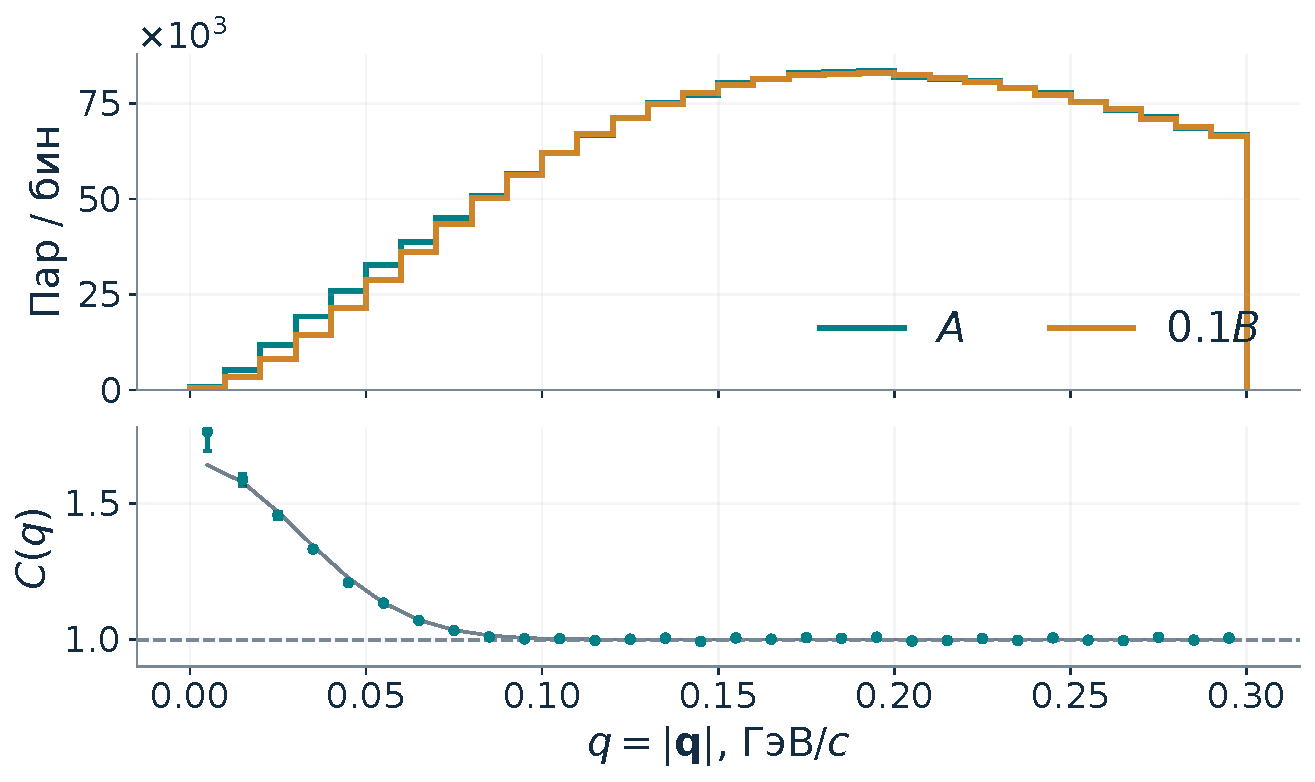
\includegraphics[width=\linewidth]{same_mixed.pdf}
\column{.32\textwidth}
$A$: пары \textbf{внутри}\par одного события.\par\vspace{2mm}
$B$: пары из \textbf{разных}\par похожих событий.
\[\boxed{C(q)=\mathcal N\frac{A(q)}{B(q)}}\]
$\mathcal N$: $C\simeq1$\par в области нормировки.
\end{columns}
\vspace{3mm}{\small\color{muted}Учебный пример: независимые пуассоновские гистограммы. Реальное смешивание событий не моделируется.\par}

\slidenote{18}
\end{frame}
\section{Что извлекаем из данных}
\begin{frame}{Три радиуса области испускания}
\begin{columns}[c,onlytextwidth]
\column{.38\textwidth}
\begin{tikzpicture}[scale=1.03]
\fill[pale] (-.9,-.7) ellipse (1.3 and .8);
\draw[arr,teal,very thick] (0,0)--(2.6,0) node[right] {out};
\draw[arr,gold,very thick] (0,0)--(-1.25,1.6) node[above] {side};
\draw[arr,ink,very thick] (0,0)--(0,-2.3) node[below] {long};
\node[font=\scriptsize,text=teal] at (1.6,-.45) {$\parallel\mathbf K_T$};
\node[font=\scriptsize] at (1.1,-2) {пучок};
\end{tikzpicture}
\column{.58\textwidth}
{\color{teal}\textbf{Система отсчёта LCMS}}\par
\small Суммарный продольный импульс пары равен нулю:
\[p_{1z}+p_{2z}=0.\]
\small Поперечное движение остаётся.\par\vspace{3mm}
\[C=1+\lambda e^{-\left(R_o^2q_o^2+R_s^2q_s^2+R_l^2q_l^2\right)/(\hc)^2}.\]
\par\vspace{2mm}
\textbf{out}: вдоль $\mathbf K_T$;\quad \textbf{long}: вдоль пучка.\par
\textbf{side}: перпендикулярно $\mathbf K_T$ и пучку.
\end{columns}


\slidenote{19}
\end{frame}
\begin{frame}{Двухпионные корреляции STAR при 3 ГэВ}
\measuretag
\vspace{3mm}
\centering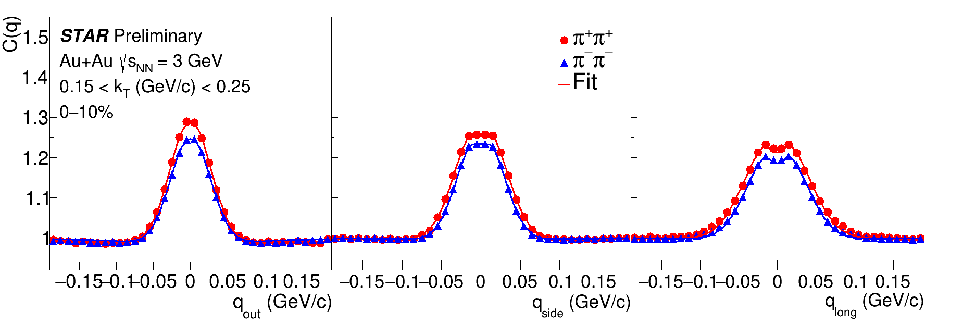
\includegraphics[width=\textwidth,height=59mm,keepaspectratio]{kraeva_2024_correlation_projections.pdf}\par
\vspace{4mm}
{\small Точки — измерения STAR.\par
Линии — аппроксимация с учётом кулоновского отталкивания.\par}
\slidenote{20}
\end{frame}
\begin{frame}{Коллективное расширение и область однородности}
\begin{columns}[c,onlytextwidth]
\column{.60\textwidth}
\begin{tikzpicture}[scale=1.05]
\fill[teal!8] (0,0) ellipse (2.3 and 1.85);
\draw[teal,thick] (0,0) ellipse (2.3 and 1.85);
\foreach \a in {0,45,...,315}{\draw[arr,teal!65] (\a:.6)--(\a:1.6);}
\fill[gold!40,opacity=.8] (1.5,.05) ellipse (.52 and .9);
\draw[gold,thick] (1.5,.05) ellipse (.52 and .9);
\foreach \y in {-.4,0,.4}{\draw[arr,gold,line width=1.4pt] (1.5,\y)--(2.9,\y);}
\node[font=\small] at (3,.8) {$\mathbf K_T$};
\node[font=\scriptsize,align=center] at (0,-2.3) {Весь источник};
\end{tikzpicture}
\column{.36\textwidth}
\prompt{Средний импульс зависит}\prompt{от места испускания.}
\vspace{3mm}
Пионы с близкими импульсами\par испускаются преимущественно\par из части системы —\par \textbf{области однородности}.\par\vspace{3mm}

\end{columns}


\slidenote{21}
\end{frame}
\begin{frame}{Радиусы STAR: зависимость от $k_T$}
\measuretag
\begin{columns}[c,onlytextwidth]
\column{.61\textwidth}\centering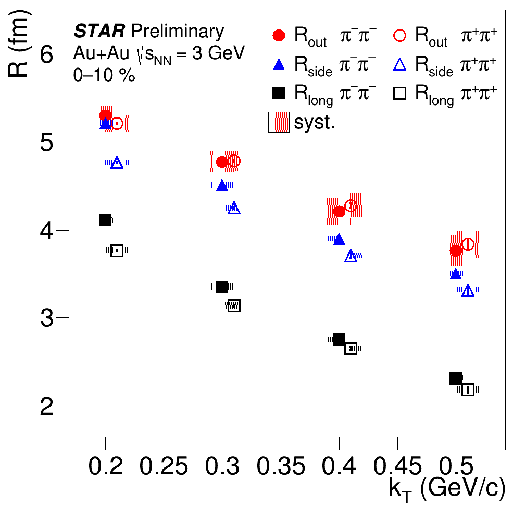
\includegraphics[width=\linewidth,height=60mm,keepaspectratio]{kraeva_2024_radii_kt.pdf}
\column{.35\textwidth}
\prompt{Радиусы уменьшаются}\prompt{при увеличении $k_T$.}
\vspace{5mm}
Какие сценарии расширения\par воспроизводят эту зависимость?
\end{columns}

\slidenote{22}
\end{frame}
\begin{frame}{Пространство и время в радиусе $R_{\rm out}$}
\begin{center}
{\large В интерференционной фазе связаны положение и время}
\vspace{5mm}
{\Large\[\boxed{R_{\rm out}^2=\left\langle\left(\widetilde x_o-\beta_T\widetilde{ct}\right)^2\right\rangle_K}\]}
\vspace{5mm}
\small $\widetilde a=a-\langle a\rangle_K$; $\beta_T$ — поперечная скорость пары в единицах $c$.
\par\vspace{3mm}
Пространство, время и их корреляция.\par
\vspace{6mm}
{\color{teal}\large Одного радиуса недостаточно для измерения длительности.\par}
\end{center}
\slidenote{23}
\end{frame}
\section{Моделирование в SMASH}
\begin{frame}{Адронная транспортная модель SMASH}
\begin{tikzpicture}[x=1cm,y=1cm]
\node[card,text width=3.2cm,minimum height=18mm] (a) at (2,0) {Ядра\\и начальные условия};
\node[card,text width=4cm,minimum height=18mm] (b) at (7.4,0) {Движение адронов,\\столкновения, распады};
\node[card,text width=3.5cm,minimum height=18mm] (c) at (13.2,0) {Точки испускания\\и импульсы\\$\{x_i^\mu,p_i^\mu\}$};
\draw[arr,teal] (a)--(b);\draw[arr,teal] (b)--(c);
\end{tikzpicture}
\vspace{6mm}
\begin{columns}[c,onlytextwidth]
\column{.49\textwidth}\tagline{В ЭКСПЕРИМЕНТЕ}\textbf{Импульсы известны.}\par Координаты испускания неизвестны.
\column{.47\textwidth}\tagline{В МОДЕЛИ}\textbf{Координаты испускания известны.}\par Можно проверить извлечение радиусов.
\end{columns}
\vspace{5mm}{\color{teal}\large SMASH моделирует адронную стадию.\par}

\slidenote{24}
\end{frame}
\begin{frame}{Расчёт корреляций по событиям SMASH}
\begin{tikzpicture}[x=1cm,y=1cm]
\node[card,text width=3.3cm] (a) at (2.1,0) {Точки испускания\\и импульсы пионов};
\node[card,text width=3cm] (b) at (7.7,0) {Группируем пары по $\mathbf q$\\$q_i,\ \Delta x_i$};
\node[card,text width=3.1cm] (c) at (13,0) {Квантовый вес\\$w_i=1+\cos\varphi_i$};
\draw[arr,teal] (a)--(b);\draw[arr,teal] (b)--(c);
\end{tikzpicture}
\vspace{7mm}
\[\varphi_i=\frac{q_i\cdot\Delta x_i}{\hc},\qquad\boxed{C_{\rm model}=\frac{\sum_iw_i}{n}}\]
\vspace{4mm}
\begin{center}\small Средний вес тех же $n$ пар. Взаимодействием пионов после испускания пренебрегаем.\end{center}
\slidenote{25}
\end{frame}
\begin{frame}{SMASH: трёхмерная корреляционная функция}
\tagline{SMASH · ТЕКУЩИЙ РАСЧЁТ · Au+Au, 3 ГэВ · $\pi^-\pi^-$ · LCMS}
\vspace{2mm}
\begin{columns}[T,onlytextwidth]
\column{.32\textwidth}\centering
{\large\color{teal}\textbf{out}\quad $C(q_{\rm out})$}\par\vspace{1mm}
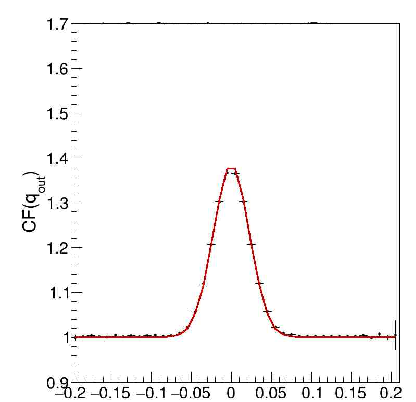
\includegraphics[width=\linewidth,height=43mm,keepaspectratio]{current_2026_cf_kt_out.pdf}\par
{\small $q_{\rm out}$, ГэВ/$c$}
\column{.32\textwidth}\centering
{\large\color{gold!80!black}\textbf{side}\quad $C(q_{\rm side})$}\par\vspace{1mm}
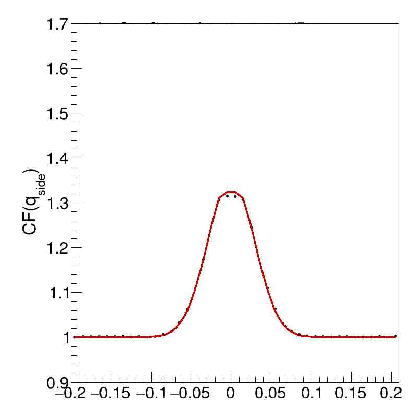
\includegraphics[width=\linewidth,height=43mm,keepaspectratio]{current_2026_cf_kt_side.pdf}\par
{\small $q_{\rm side}$, ГэВ/$c$}
\column{.32\textwidth}\centering
{\large\color{ink}\textbf{long}\quad $C(q_{\rm long})$}\par\vspace{1mm}
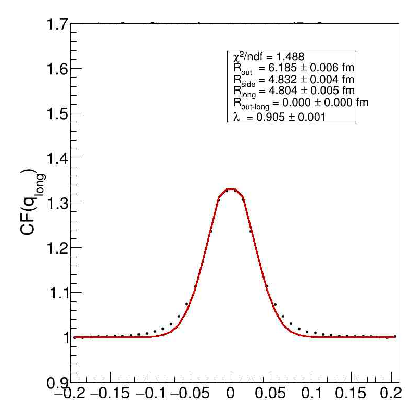
\includegraphics[width=\linewidth,height=43mm,keepaspectratio]{current_2026_cf_kt_long.pdf}\par
{\small $q_{\rm long}$, ГэВ/$c$}
\end{columns}
\vspace{2mm}
\begin{center}\small Центральность 0–10\%; $0.15<k_T<0.25$ ГэВ/$c$.\end{center}


\slidenote{26}
\end{frame}
\begin{frame}{SMASH: поперечные радиусы $R_{\rm out}$ и $R_{\rm side}$, фм}
\tagline{SMASH · ТЕКУЩИЙ РАСЧЁТ · Au+Au, 3 ГэВ · $\pi^-\pi^-$ · LCMS}
\vspace{2mm}
\begin{columns}[T,onlytextwidth]
\column{.48\textwidth}\centering
{\large\color{teal}$R_{\rm out}$, фм}\par
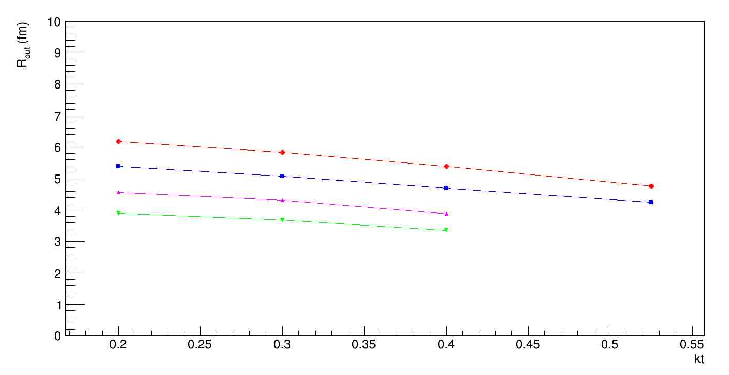
\includegraphics[width=\linewidth,height=57mm,keepaspectratio]{current_2026_kt_out.pdf}
\column{.48\textwidth}\centering
{\large\color{gold!80!black}$R_{\rm side}$, фм}\par
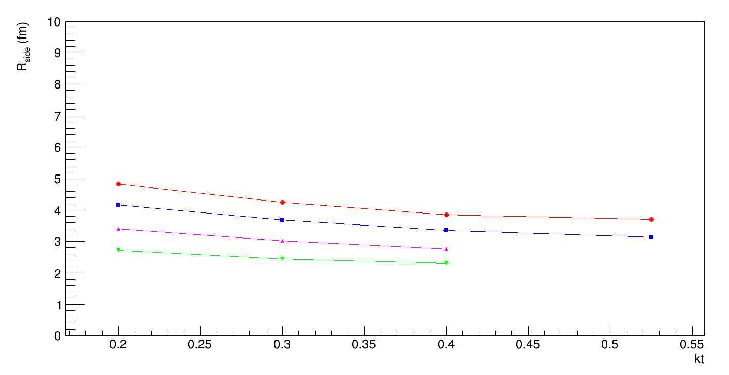
\includegraphics[width=\linewidth,height=57mm,keepaspectratio]{current_2026_kt_side.pdf}
\end{columns}
\par\vspace{1mm}{\centering\small $k_T$, ГэВ/$c$\par\vspace{1mm}Центральность:\quad \textcolor{red!75!black}{0–10\%}\quad \textcolor{blue!75!black}{10–30\%}\quad \textcolor{magenta!75!black}{30–50\%}\quad \textcolor{green!35!black}{50–80\%}\par}


\slidenote{27}
\end{frame}
\begin{frame}{SMASH: продольный радиус $R_{\rm long}$}
\begin{columns}[c,onlytextwidth]
\column{.65\textwidth}\centering
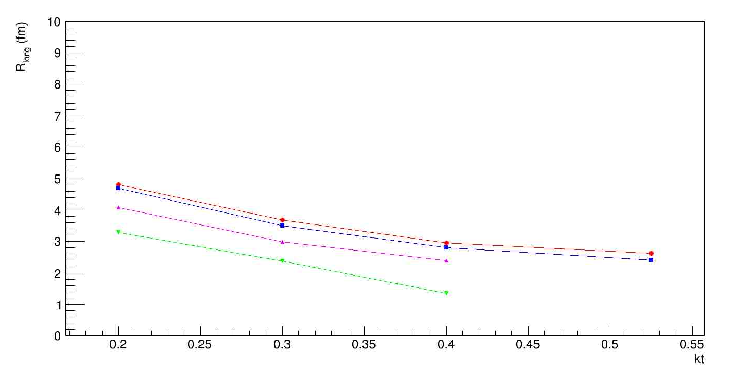
\includegraphics[width=\linewidth,height=60mm,keepaspectratio]{current_2026_kt_long.pdf}
\column{.31\textwidth}
\tagline{SMASH · ТЕКУЩИЙ РАСЧЁТ}
{\large $R_{\rm long}(k_T)$, фм}\par
\small $\pi^-\pi^-$ · LCMS\par $k_T$, ГэВ/$c$\par\vspace{4mm}
\small Центральность:\par\vspace{1mm}
\textcolor{red!75!black}{0–10\%}\par
\textcolor{blue!75!black}{10–30\%}\par
\textcolor{magenta!75!black}{30–50\%}\par
\textcolor{green!35!black}{50–80\%}
\end{columns}


\slidenote{28}
\end{frame}
\begin{frame}{Сравнение радиусов SMASH и STAR}
\tagline{Au+Au · $\sqrt{s_{NN}}=3$ ГэВ · 0–10\% · $\pi^-\pi^-$ · LCMS}
\vspace{1mm}
\centering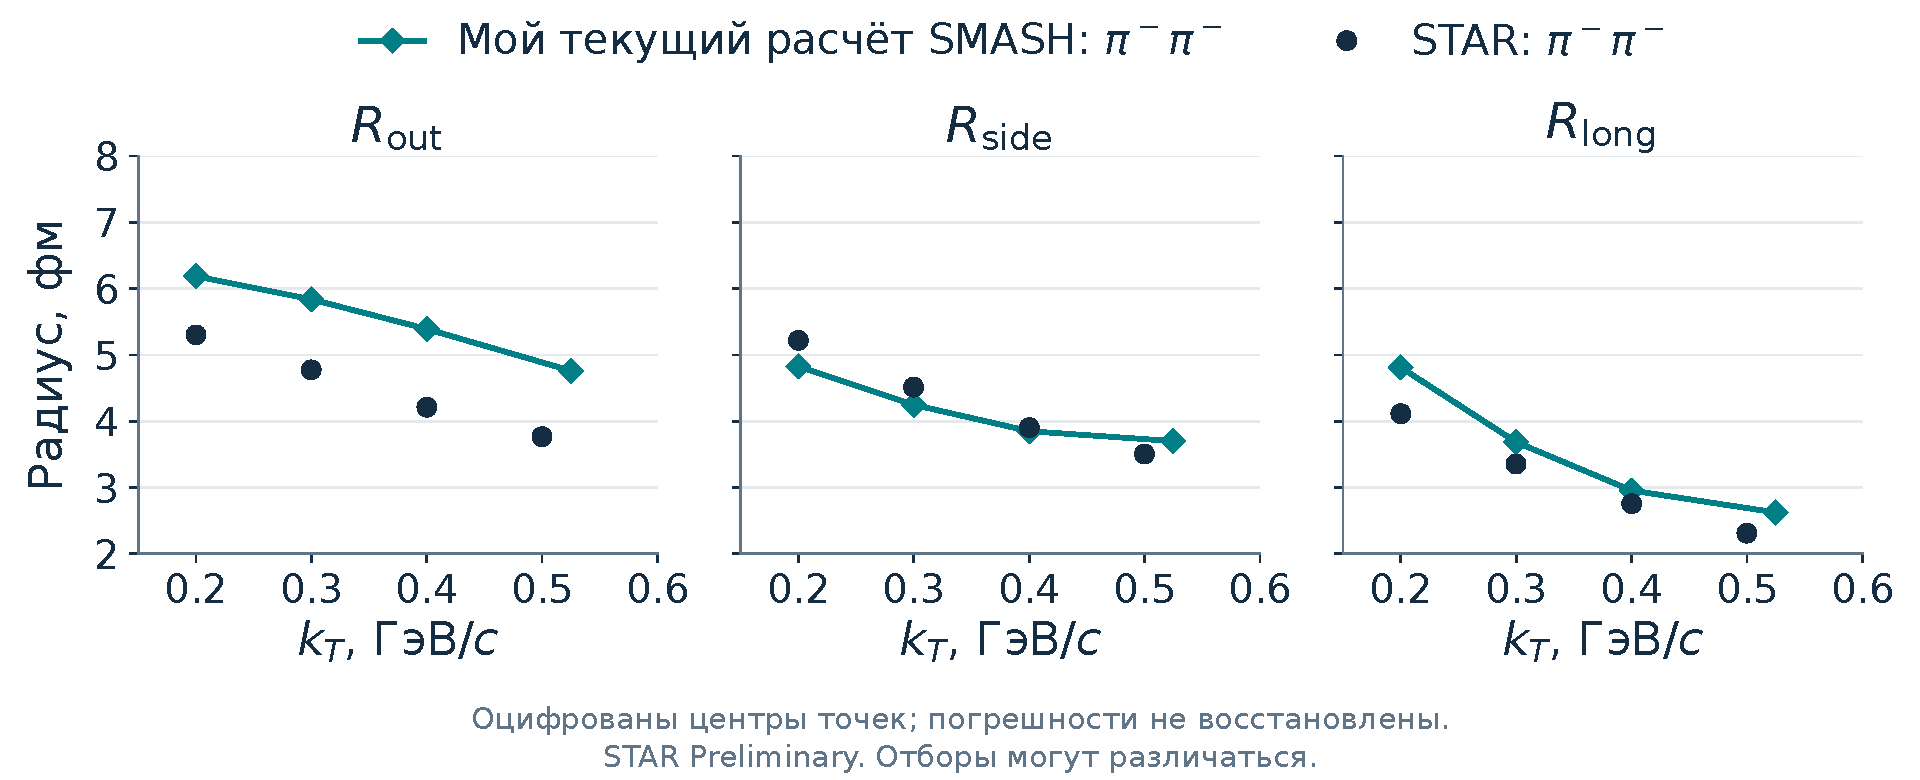
\includegraphics[width=\textwidth,height=65mm,keepaspectratio]{comparison_star_smash_current_2026.pdf}\par
\slidenote{29}
\end{frame}
\section{Результаты и интерпретация}
\begin{frame}{Корреляции пионов характеризуют область испускания}
\begin{columns}[T,onlytextwidth]
\column{.29\textwidth}
\prompt{Детекторы}
\vspace{4mm}
TPC + TOF\par\vspace{2mm}
Импульсы и виды частиц.
\column{.31\textwidth}
\prompt{Корреляция}
\vspace{4mm}
Корреляция $C(q)$\par\vspace{2mm}
Ширина пика $\to$\par масштаб испускания.
\column{.31\textwidth}
\prompt{Область испускания}
\vspace{4mm}
Радиусы и их зависимости\par\vspace{2mm}
Модели расширения\par плотной материи.
\end{columns}
\vspace{7mm}
\begin{center}\large\color{teal}Парные корреляции дополняют одночастичные спектры.\end{center}
\slidenote{30}
\end{frame}
\appendix
\section{Источники и резерв}
\begin{frame}{Литература: теория, STAR и SMASH}
\small
\textbf{Lisa, Pratt, Soltz, Wiedemann (2005).}\par
Формализм, области однородности, методы анализа.\par
\href{https://arxiv.org/abs/nucl-ex/0505014}{arXiv:nucl-ex/0505014}\par\vspace{2mm}
\textbf{Anna Kraeva for STAR. Universe 10, 188 (2024).}\par
\emph{Two-Pion Bose–Einstein Correlations in Au+Au Collisions at $\sqrt{s_{NN}}=3$ GeV in the STAR Experiment.}\par
\href{https://doi.org/10.3390/universe10040188}{DOI: 10.3390/universe10040188}\quad
\href{https://indico.cern.ch/event/1258038/contributions/5537099/attachments/2700455/4687127/ISMD_2023_v6.pdf}{Доклад ISMD 2023}\par\vspace{2mm}
\textbf{Weil et al. PRC 94, 054905 (2016).}\par
SMASH: \href{https://arxiv.org/abs/1606.06642}{arXiv:1606.06642},
\href{https://smash-transport.github.io/}{официальная документация}.\par\vspace{2mm}
\textbf{STAR. PRC 71, 044906 (2005).}\quad\href{https://arxiv.org/abs/nucl-ex/0411036}{Методика и детекторные эффекты.}

\slidenote{31}
\end{frame}
\begin{frame}{Литература: история метода и детекторы}
\small
\textbf{Hanbury Brown, Twiss (1956): корреляции и Сириус.}\par
\href{https://doi.org/10.1038/177027a0}{Nature 177, 27–29};\quad
\href{https://doi.org/10.1038/1781046a0}{Nature 178, 1046–1048}.\par\vspace{2mm}
\textbf{Goldhaber, Goldhaber, Lee, Pais (1960): пионы.}\par
\href{https://doi.org/10.1103/PhysRev.120.300}{Phys. Rev. 120, 300–312.}\par\vspace{2mm}
\textbf{Копылов–Подгорецкий (1972); Копылов (1974).}\par
ЯФ 15, 392;\quad\href{https://doi.org/10.1016/0370-2693(74)90263-9}{Phys. Lett. B 50, 472–474}.\par\vspace{2mm}
\textbf{Anderson et al.: STAR TPC.}\quad\href{https://arxiv.org/abs/nucl-ex/0301015}{nucl-ex/0301015}.\par
\textbf{Shao et al.: совместная идентификация.}\quad\href{https://arxiv.org/abs/nucl-ex/0505026}{nucl-ex/0505026}.\par
\textbf{Llope et al.: STAR TOFp.}\quad\href{https://arxiv.org/abs/nucl-ex/0308022}{nucl-ex/0308022}.

\slidenote{32}
\end{frame}
\begin{frame}{Работы автора: архив 2023–2025}
\begin{columns}[T,onlytextwidth]
\column{.50\textwidth}\small
\textbf{Балинов, 2023:} полный текст, 21 стр.\par
\href{https://epp.phys.msu.ru/kr2kurs}{Архив кафедры, 2 курс}. Обзор метода.\par\vspace{2mm}
\textbf{Балинов, 2025:} защита, 28 слайдов.\par
\href{https://epp.phys.msu.ru/kr4kurs}{Архив кафедры, 4 курс}. Модельные графики.\par\vspace{2mm}
Число событий, версия SMASH,\par способ оценки погрешностей\par и программа подгонки\par по архиву не установлены.\par\vspace{2mm}
В исходных формулах есть ошибки\par размерностей и знаков; реализация\par 2025 года не проверена.
\column{.46\textwidth}\small
\begin{tabular}{@{}ll@{}}\toprule
Система & Au+Au, 3 ГэВ\\
Пары & $\pi^+\pi^+$, $\pi^-\pi^-$\\
$|\mathbf p|,p_T$ & 0.15–1.5 ГэВ/$c$\\
$\eta$ & $[-1.5,1.5]$\\
$k_T$ & 0.15–0.25; 0.25–0.35;\\
(ГэВ/$c$) & 0.35–0.45; 0.45–0.60\\
Центральность & 0–10; 10–30;\\
 & 30–50; 50–80\%\\\bottomrule\end{tabular}
\end{columns}

\slidenote{33}
\end{frame}
\begin{frame}{Расчёт 2025 года: одномерная корреляция}
\begin{columns}[c,onlytextwidth]
\column{.68\textwidth}\centering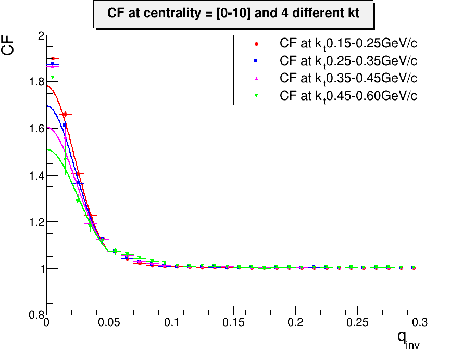
\includegraphics[width=\linewidth,height=61mm,keepaspectratio]{balinov_2025_correlation_kt.pdf}
\column{.28\textwidth}
\tagline{SMASH / АРХИВ 2025}
\textbf{Au+Au, 3 ГэВ}\par Центральность 0–10\%.\par\vspace{3mm}
\small $q_{\rm inv}$ — инвариантная\par мера различия импульсов.\par
В покое пары: $q_{\rm inv}=2|\mathbf p^*|$.\par\vspace{2mm} Четыре интервала $k_T$:\par
\textcolor{red}{0.15–0.25}\par
\textcolor{blue}{0.25–0.35}\par
\textcolor{magenta}{0.35–0.45}\par
\textcolor{green!45!black}{0.45–0.60}\par ГэВ/$c$.
\end{columns}
\takeaway{Отбор по импульсу пары входит в определение измеряемого источника.}

\slidenote{34}
\end{frame}
\begin{frame}{Расчёт 2025 года: радиус $R_{\rm inv}$}
\begin{columns}[c,onlytextwidth]
\column{.68\textwidth}\centering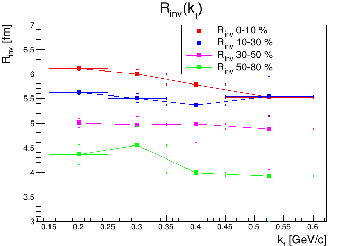
\includegraphics[width=\linewidth,height=58mm,keepaspectratio]{balinov_2025_rinv.pdf}
\column{.28\textwidth}
\tagline{SMASH / АРХИВ 2025}
\textbf{$R_{\rm inv}(k_T)$}\par параметр одномерной\par аппроксимации.\par\vspace{3mm}
\small \textcolor{red}{0–10\%}\par
\textcolor{blue}{10–30\%}\par
\textcolor{magenta}{30–50\%}\par
\textcolor{green!45!black}{50–80\%}\par\vspace{3mm}
Радиус зависит\par от центральности.
\end{columns}
\takeaway{Программа подгонки и способ оценки погрешностей не проверены.}

\slidenote{35}
\end{frame}
\begin{frame}{Смешанный член корреляции и быстрота пары}
\measuretag
\begin{columns}[c,onlytextwidth]
\column{.55\textwidth}\centering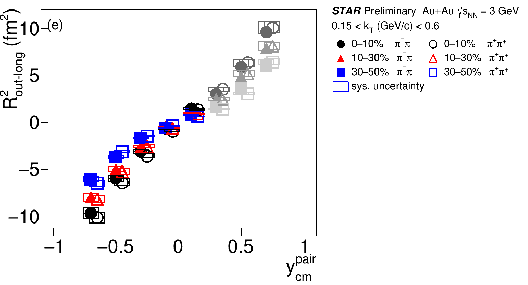
\includegraphics[width=\linewidth,height=52mm,keepaspectratio]{kraeva_2024_rapidity_out_long.pdf}\par
{\scriptsize Серые точки — зеркальное отражение данных.}
\column{.41\textwidth}
\tagline{БЫСТРОТА ПАРЫ В СИСТЕМЕ ЦЕНТРА МАСС}
\[y_{\rm pair}=\frac12\ln\frac{E_{\rm pair}+P_z}{E_{\rm pair}-P_z}.\]
\small Система центра масс столкновения.\par В LCMS переходим для каждой пары.\par\vspace{1mm}
В гауссовой экспоненте возникает\par смешанный член:
\[\color{teal}-\frac{2q_o q_l R_{ol}^2}{(\hc)^2}.\]
\small $R_{ol}^2$ — коэффициент \textbf{со знаком},\par а не квадрат положительной длины.
\end{columns}
\takeaway{Смешанный член out–long связан с продольным расширением.}

\slidenote{36}
\end{frame}
\begin{frame}{Обозначения импульсов и системы отсчёта}
\begin{columns}[c,onlytextwidth]
\column{.53\textwidth}
\tagline{ПОЛНАЯ РАЗНОСТЬ И ПОЛУСУММА}
\[\boxed{q^\mu=p_1^\mu-p_2^\mu},\qquad K^\mu=\frac{p_1^\mu+p_2^\mu}{2}.\]
\[p_i^\mu=(E_i,\mathbf p_i),\qquad c=1.\]
\[q_{\rm inv}=\sqrt{|\mathbf q|^2-(q^0)^2}.\]
\small В покое пары: $q^0=0$,\par $q_{\rm inv}=2|\mathbf p_1^*|$ для равных масс.
\column{.43\textwidth}
\begin{tikzpicture}[scale=1.0]
\draw[arr,teal,line width=1.7pt] (0,0)--(3,1.4) node[right] {$\mathbf p_{1T}$};
\draw[arr,gold,line width=1.7pt] (0,0)--(2.5,.3) node[right] {$\mathbf p_{2T}$};
\draw[arr,ink] (2.5,.3)--(3,1.4) node[midway,right=1.5mm] {$\mathbf q_T$};
\draw[arr,ink,dashed] (0,0)--(2.75,.85);
\node[font=\small] at (1.6,-.55) {Пунктир: $\mathbf K_T$};
\end{tikzpicture}
\[k_T=\frac{|\mathbf p_{1T}+\mathbf p_{2T}|}{2}.\]

\end{columns}

\slidenote{37}
\end{frame}
\begin{frame}{STAR: столкновения с неподвижной мишенью}
\measuretag
\begin{columns}[c,onlytextwidth]
\column{.60\textwidth}
\begin{tikzpicture}[x=1cm,y=1cm]
\fill[pale,rounded corners] (.3,-1.5) rectangle (9,1.7);
\draw[teal!40,thick] (.3,-1.5) rectangle (9,1.7);
\node[teal,font=\small\bfseries] at (4.7,2.1) {STAR: неподвижная мишень (FXT)};
\draw[arr,ink,very thick] (-.3,0)--(1.9,0) node[midway,above] {пучок Au};
\draw[gold,line width=4pt] (2.1,-.5)--(2.1,.5);
\node[below,font=\scriptsize] at (2.1,-.55) {мишень Au};
\foreach \y in {-1.1,-.4,.4,1.1}{\draw[teal,line width=1.1pt] (2.1,0) to[out=10,in=180] (8.4,\y);}
\node[font=\small] at (6.8,-1.1) {TPC + TOF};
\node[align=center,font=\scriptsize,text=muted] at (4.7,-2.4) {Продольная схема, без масштаба\\мишень у края детектора, а не в его центре};
\end{tikzpicture}
\column{.36\textwidth}
\chip{\linewidth}{Кривизна трека $\to p_T$}\par\vspace{2mm}
\chip{\linewidth}{$dE/dx$ и время пролёта $\to\pi$}\par\vspace{3mm}
\textbf{Импульс — измеряем.}\par
Масштабы области\par испускания — оцениваем\par статистически.
\end{columns}

\slidenote{38}
\end{frame}
\begin{frame}{STAR: отбор пионов и область регистрации}
\measuretag
\begin{columns}[c,onlytextwidth]
\column{.47\textwidth}\centering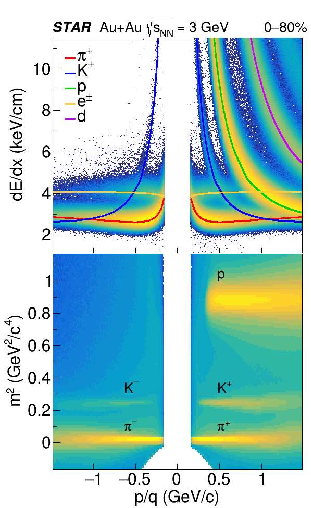
\includegraphics[width=\linewidth,height=58mm,keepaspectratio]{kraeva_2024_pid.pdf}
\column{.49\textwidth}\centering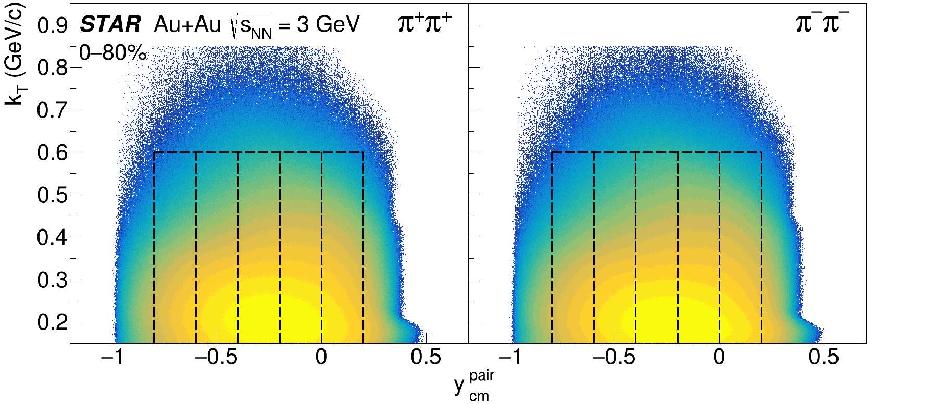
\includegraphics[width=\linewidth,height=50mm,keepaspectratio]{kraeva_2024_acceptance.pdf}\par
\small $y_{\rm pair}$ — быстрота пары;\par $\eta$ — псевдобыстрота отдельного пиона.
\end{columns}

\slidenote{39}
\end{frame}
\begin{frame}{Фазовая диаграмма и область 3 ГэВ}
\begin{columns}[c,onlytextwidth]
\column{.64\textwidth}
\begin{tikzpicture}[x=1cm,y=1cm]
\fill[teal!7] (0,3.5) .. controls (2.5,3.5) and (5,3) .. (7.2,1.8) -- (7.2,5) -- (0,5) -- cycle;
\fill[gold!12] (5.6,.1) rectangle (7.2,4.95);
\draw[arr,ink] (0,0)--(7.7,0);
\draw[arr,ink] (0,0)--(0,5.4) node[above right] {$T$};
\draw[teal,very thick] (0,3.5) .. controls (1.0,3.5) and (1.7,3.5) .. (2.4,3.35);
\draw[teal,very thick,dashed] (2.4,3.35) .. controls (4,3.2) and (5.5,2.8) .. (7.2,1.8);
\node[font=\small,align=center] at (3.1,4.35) {Кварк-глюонная\\плазма};
\node[font=\small,align=center] at (2.7,1.7) {Адронная\\материя};
\node[font=\small,text=gold!75!black,align=center] at (6.4,.9) {STAR FXT\\3 ГэВ};
\node[font=\scriptsize,text=muted] at (4.7,3.5) {Переход?};
\node[font=\small,align=center] at (3.8,-.65) {Барионный химический потенциал $\mu_B$};
\node[font=\scriptsize,text=muted] at (3.7,-1.25) {Качественная схема};
\end{tikzpicture}
\column{.32\textwidth}
\prompt{Материя с высокой}\prompt{барионной плотностью.}
\vspace{6mm}
Как она расширяется\par и испускает частицы?
\end{columns}
\slidenote{40}
\end{frame}
\begin{frame}{Расчёт 2025 года: трёхмерная корреляция}
\tagline{SMASH · РАСЧЁТ 2025 · Au+Au, 3 ГэВ}
\vspace{2mm}
\begin{columns}[T,onlytextwidth]
\column{.32\textwidth}\centering
{\large\color{teal}\textbf{out}\quad $C(q_{\rm out})$}\par\vspace{1mm}
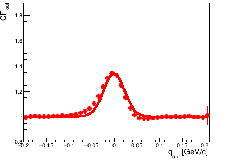
\includegraphics[width=\linewidth,height=38mm,keepaspectratio]{balinov_2025_correlation_out_3d.pdf}\par
{\small $q_{\rm out}$, ГэВ/$c$}
\column{.32\textwidth}\centering
{\large\color{gold!80!black}\textbf{side}\quad $C(q_{\rm side})$}\par\vspace{1mm}
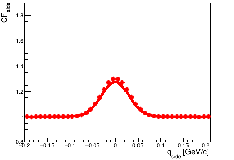
\includegraphics[width=\linewidth,height=38mm,keepaspectratio]{balinov_2025_correlation_side_3d.pdf}\par
{\small $q_{\rm side}$, ГэВ/$c$}
\column{.32\textwidth}\centering
{\large\color{ink}\textbf{long}\quad $C(q_{\rm long})$}\par\vspace{1mm}
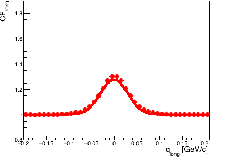
\includegraphics[width=\linewidth,height=38mm,keepaspectratio]{balinov_2025_correlation_long_3d.pdf}\par
{\small $q_{\rm long}$, ГэВ/$c$}
\end{columns}
\vspace{2mm}
\begin{center}\small Центральность 0–10\%; $0.15<k_T<0.25$ ГэВ/$c$.\end{center}


\slidenote{41}
\end{frame}
\begin{frame}{Расчёт 2025 года: поперечные радиусы}
\tagline{SMASH · РАСЧЁТ 2025 · Au+Au, 3 ГэВ}
\vspace{2mm}
\begin{columns}[T,onlytextwidth]
\column{.48\textwidth}\centering
{\large\color{teal}$R_{\rm out}$}\par
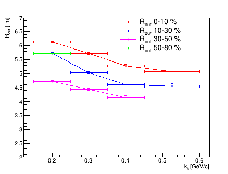
\includegraphics[width=\linewidth,height=57mm,keepaspectratio]{balinov_2025_rout_3d.pdf}
\column{.48\textwidth}\centering
{\large\color{gold!80!black}$R_{\rm side}$}\par
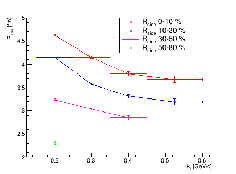
\includegraphics[width=\linewidth,height=57mm,keepaspectratio]{balinov_2025_rside_3d.pdf}
\end{columns}
\par\vspace{1mm}{\centering\small Центральность:\quad \textcolor{red!75!black}{0–10\%}\quad \textcolor{blue!75!black}{10–30\%}\quad \textcolor{magenta!75!black}{30–50\%}\quad \textcolor{green!35!black}{50–80\%}\par}


\slidenote{42}
\end{frame}
\begin{frame}{Расчёт 2025 года: продольный радиус}
\begin{columns}[c,onlytextwidth]
\column{.65\textwidth}\centering
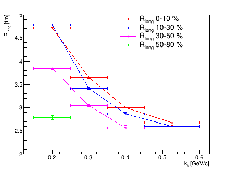
\includegraphics[width=\linewidth,height=60mm,keepaspectratio]{balinov_2025_rlong_3d.pdf}
\column{.31\textwidth}
\tagline{SMASH · РАСЧЁТ 2025}
{\large $R_{\rm long}(k_T)$}\par\vspace{5mm}
\small Центральность:\par\vspace{1mm}
\textcolor{red!75!black}{0–10\%}\par
\textcolor{blue!75!black}{10–30\%}\par
\textcolor{magenta!75!black}{30–50\%}\par
\textcolor{green!35!black}{50–80\%}
\end{columns}


\slidenote{43}
\end{frame}
\begin{frame}{SMASH: корреляции в интервале быстроты 0–0,2}
\tagline{SMASH · ТЕКУЩИЙ РАСЧЁТ · Au+Au, 3 ГэВ · $\pi^-\pi^-$ · LCMS}
\vspace{2mm}
\begin{columns}[T,onlytextwidth]
\column{.32\textwidth}\centering
{\large\color{teal}\textbf{out}\quad $C(q_{\rm out})$}\par\vspace{1mm}
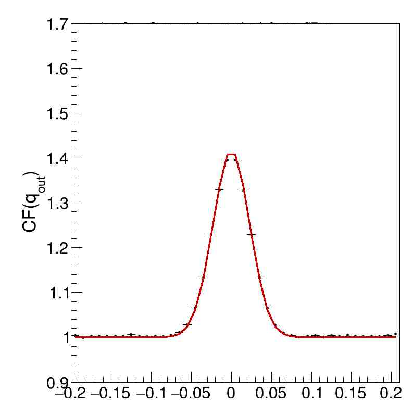
\includegraphics[width=\linewidth,height=43mm,keepaspectratio]{current_2026_cf_y_out.pdf}\par
{\small $q_{\rm out}$, ГэВ/$c$}
\column{.32\textwidth}\centering
{\large\color{gold!80!black}\textbf{side}\quad $C(q_{\rm side})$}\par\vspace{1mm}
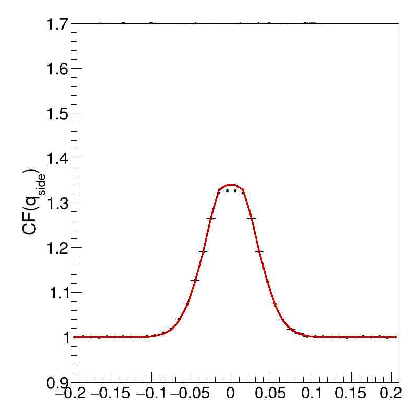
\includegraphics[width=\linewidth,height=43mm,keepaspectratio]{current_2026_cf_y_side.pdf}\par
{\small $q_{\rm side}$, ГэВ/$c$}
\column{.32\textwidth}\centering
{\large\color{ink}\textbf{long}\quad $C(q_{\rm long})$}\par\vspace{1mm}
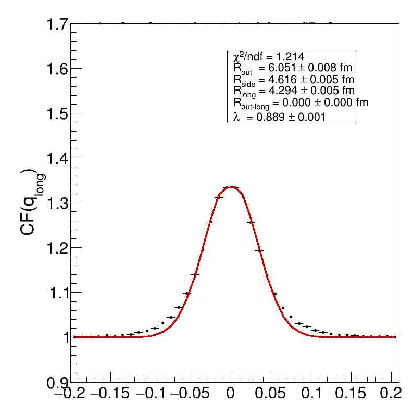
\includegraphics[width=\linewidth,height=43mm,keepaspectratio]{current_2026_cf_y_long.pdf}\par
{\small $q_{\rm long}$, ГэВ/$c$}
\end{columns}
\vspace{2mm}
\begin{center}\small Центральность 0–10\%; $y\in[0,0.2]$ в системе центра масс Au+Au.\end{center}


\slidenote{44}
\end{frame}
\begin{frame}{SMASH: радиусы по быстроте}
\tagline{ТЕКУЩИЙ РАСЧЁТ · Au+Au, 3 ГэВ · $\pi^-\pi^-$ · LCMS}
\begin{columns}[T,onlytextwidth]
\column{.32\textwidth}\centering
{\large\color{teal}$R_{\rm out}$, фм}\par
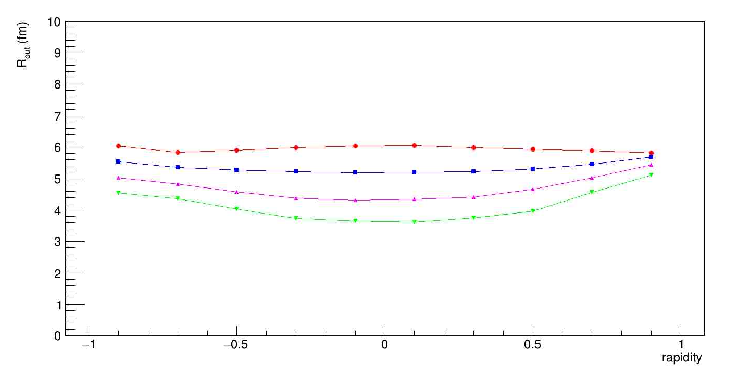
\includegraphics[width=\linewidth]{current_2026_y_out.pdf}
\column{.32\textwidth}\centering
{\large\color{gold!80!black}$R_{\rm side}$, фм}\par
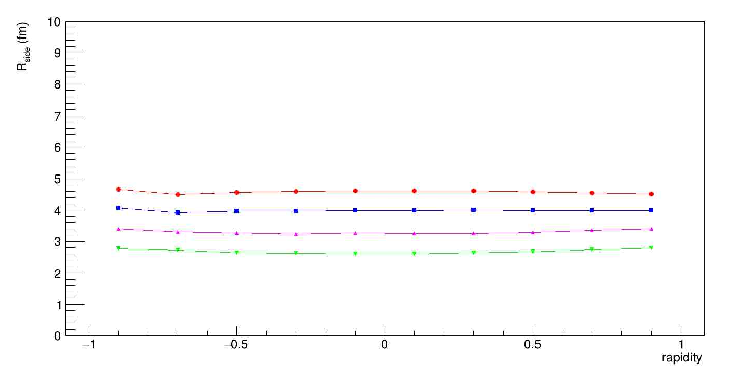
\includegraphics[width=\linewidth]{current_2026_y_side.pdf}
\column{.32\textwidth}\centering
{\large\color{ink}$R_{\rm long}$, фм}\par
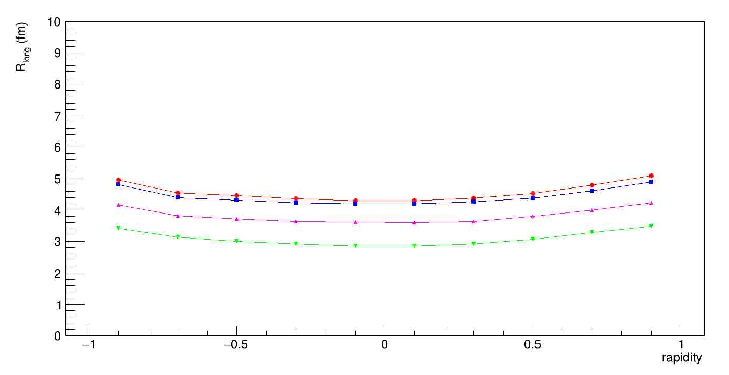
\includegraphics[width=\linewidth]{current_2026_y_long.pdf}
\end{columns}
\begin{center}\small Быстрота пары в системе центра масс: $-1<y<1$, шаг 0.2.\end{center}
{\centering\small Центральность:\quad \textcolor{red!75!black}{0–10\%}\quad \textcolor{blue!75!black}{10–30\%}\quad \textcolor{magenta!75!black}{30–50\%}\quad \textcolor{green!35!black}{50–80\%}\par}
\slidenote{45}
\end{frame}
\begin{frame}{SMASH: параметр $\lambda$}
\tagline{ТЕКУЩИЙ РАСЧЁТ · Au+Au, 3 ГэВ · $\pi^-\pi^-$ · LCMS}
\begin{columns}[T,onlytextwidth]
\column{.48\textwidth}\centering
{\large $\lambda(k_T)$}\par
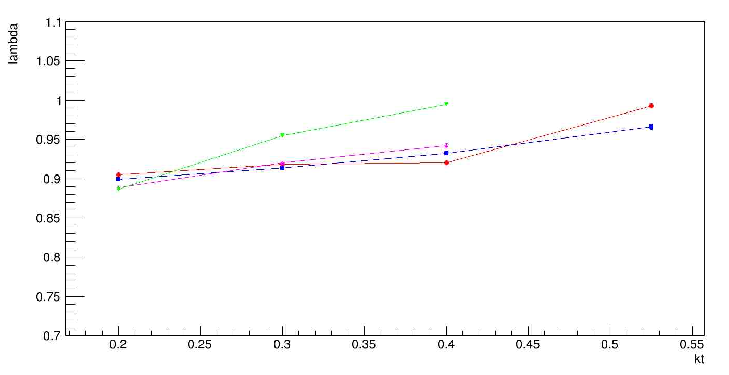
\includegraphics[width=\linewidth]{current_2026_kt_lambda.pdf}\par
{\small $k_T$, ГэВ/$c$}
\column{.48\textwidth}\centering
{\large $\lambda(y)$}\par
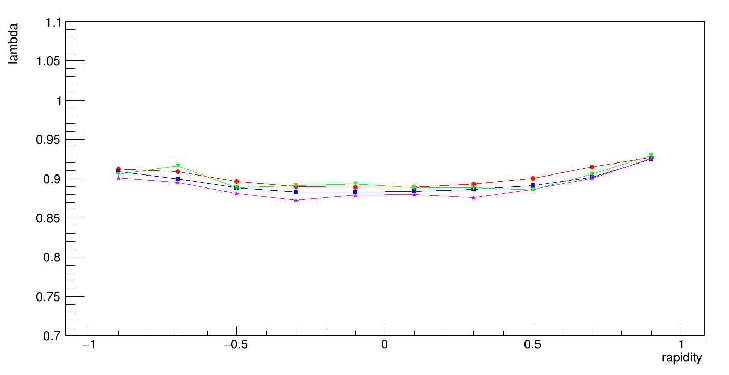
\includegraphics[width=\linewidth]{current_2026_y_lambda.pdf}\par
{\small $y$ в системе центра масс}
\end{columns}
\vspace{3mm}
{\centering\small Центральность:\quad \textcolor{red!75!black}{0–10\%}\quad \textcolor{blue!75!black}{10–30\%}\quad \textcolor{magenta!75!black}{30–50\%}\quad \textcolor{green!35!black}{50–80\%}\par}
\slidenote{46}
\end{frame}
\begin{frame}{Сравнение радиусов SMASH 2025 и STAR}
\tagline{Au+Au · $\sqrt{s_{NN}}=3$ ГэВ · 0–10\% · LCMS}
\vspace{1mm}
\centering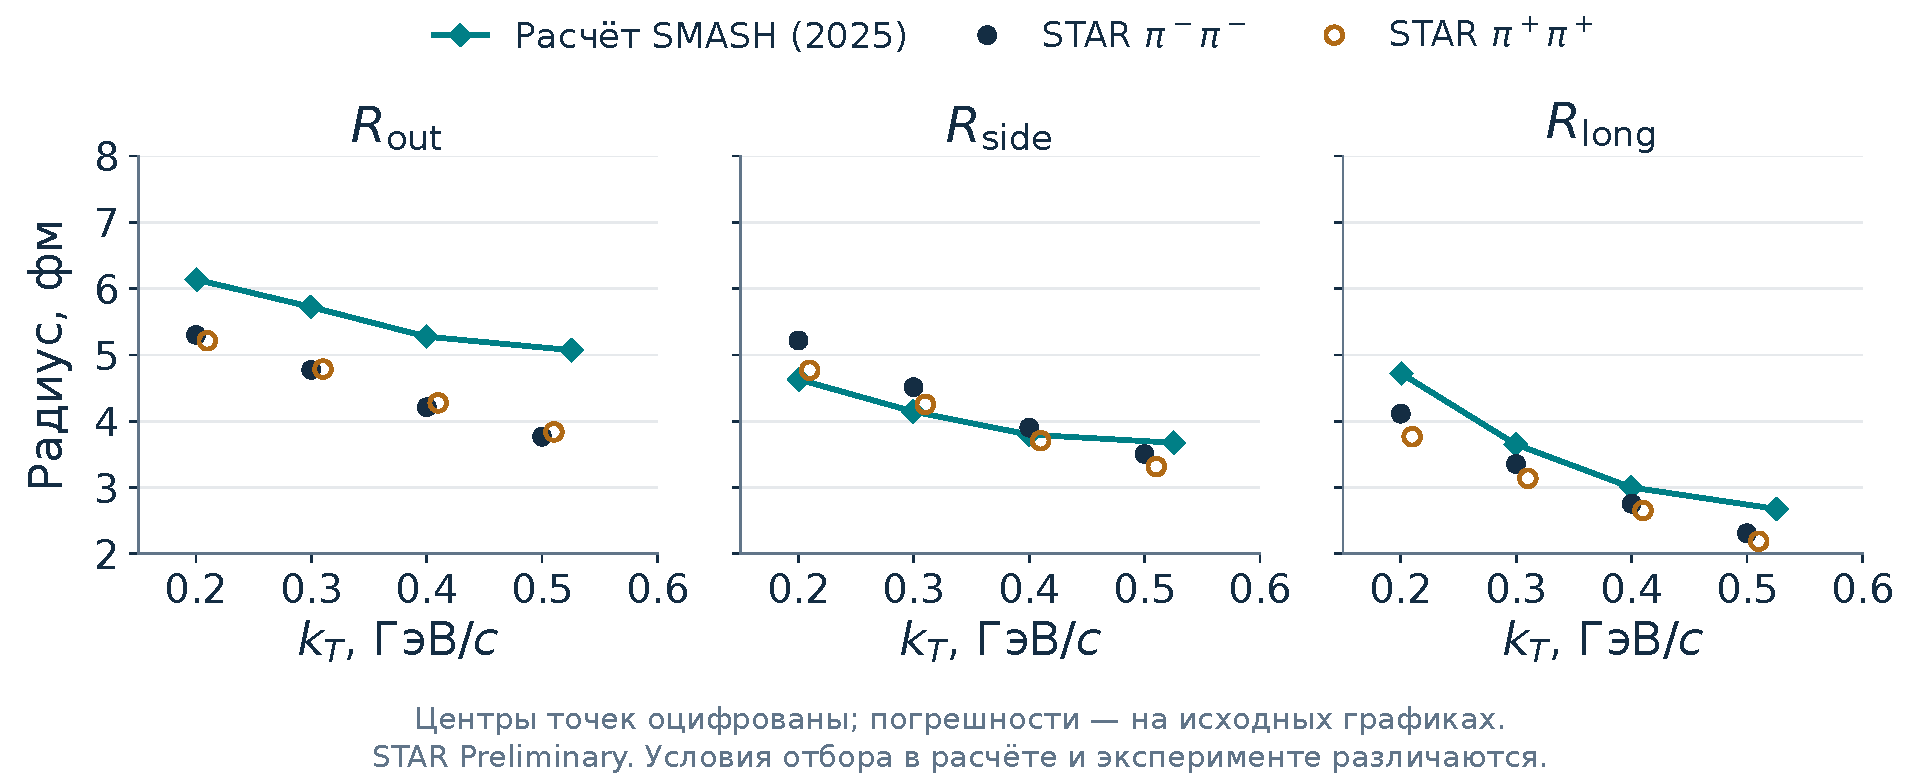
\includegraphics[width=\textwidth,height=65mm,keepaspectratio]{comparison_star_smash_2025.pdf}\par
\slidenote{47}
\end{frame}
\end{document}
